\subsection{Hachage}

\begin{frame}{Fonction de hachage : définition}
  \begin{columns}
    \begin{column}{0.7\textwidth}
      Comment appliquer cette logique à de l'information binaire ?
      On cherche une somme de contrôle universelle capable de fonctionner sur tout $\mathbb{B}$.

      $\Rightarrow$ on les appelle fonction de hachage

      \begin{block}{Définition : fonction de hachage}
        Une fonction de hachage permet de générer un \textquote{hash} de n'importe quel mot binaire.
      \end{block}

      \begin{block}{Définition : hash}
        Un hash est un mot binaire de taille fixe, dont la taille est spécifique à la fonction de hachahe utilisé.
      \end{block}
    \end{column}
    \begin{column}{0.2\textwidth}
      \resizebox{\textwidth}{!}{
        
\includegraphics{img/meat-grinder.png}
      }
    \end{column}
  \end{columns}
\end{frame}

\begin{frame}[fragile]{Fonction de hachage : exemples}
  \begin{figure}
  \begin{minted}{text}
    >>> import hashlib
    >>> hashlib.md5(b"Mathieu").hexdigest()
    '206299fa740a4327a61b67b6be5c8373'
  \end{minted}

  \caption{Calcul d'un MD5 en ligne de commande en Python}
  \label{code:md5-hash-cli}
\end{figure}
  \begin{figure}
  \begin{minted}{text}
    >>> import hashlib
    >>> hashlib.sha256(b"Mathieu").hexdigest()
    'f5e088d29801ebb822251d7751bc4b8ff28c50132d8b0a95614b5f048a1d01b6'
  \end{minted}

  \caption{Calcul d'un SHA-256 en ligne de commande en Python}
  \label{code:sha256-hash-cli}
\end{figure}
\end{frame}

\begin{frame}{Caractéristiques d'une fonction de hachage}
  \begin{block}{Uniformité}
    Une bonne fonction de hachage doit répartir uniformément les valeurs d'entrée sur l'ensemble des valeurs de hachage possibles. Cela signifie que des entrées différentes doivent avoir une probabilité égale de générer des valeurs de hachage différentes.
  \end{block}

  \begin{block}{Déterminisme}
    Pour une même valeur d'entrée, la fonction de hachage doit toujours générer la même valeur de hachage. Cela permet d'obtenir des résultats cohérents et reproductibles.
  \end{block}
\end{frame}

\begin{frame}{Caractéristiques d'une fonction de hachage}
  \begin{block}{Résistance aux collisions}
    Une fonction de hachage $h$ de taille $n$ entraîne obligatoirement des collisions car la taille de $\mathbb{B}$ est infinie alors que $\mathbb{B}_n$ n'est \textquote{que} de $2^n$.
    Une collision existe quand deux mots binaires $a$ et $b$ engendrent le même hash, c'est-à-dire :

    $$h(a) = h(b)$$

    $\Rightarrow$ une \textquote{bonne} fonction de hachage ne possède pas de hash connu.

    \begin{small}
      \textit{Note : Les algorithmes md4, md5 et sha1 ne sont à jour plus considérés comme sûrs.}
    \end{small}
  \end{block}
\end{frame}

\begin{frame}{Caractéristiques d'une fonction de hachage}
  \begin{block}{Sensibilité aux changements}
    Une petite modification dans l'entrée doit entraîner un changement significatif dans la valeur de hachage.
    Cela garantit que des entrées similaires génèrent des valeurs de hachage différentes.
  \end{block}

  \begin{figure}
  \resizebox{\columnwidth}{!}{%
    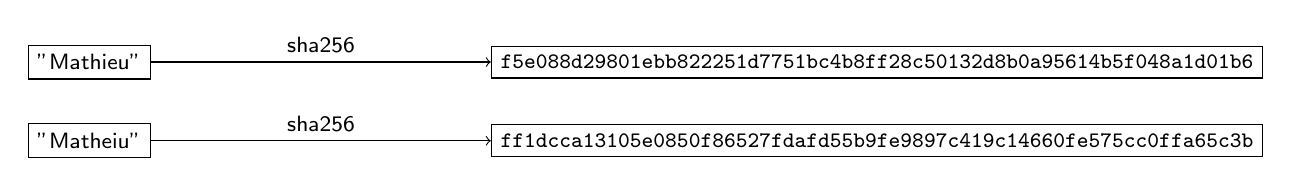
\begin{tikzpicture}[font=\sffamily\footnotesize,
        Input/.style={shape=rectangle,draw},
        Output/.style={shape=rectangle,draw}
      ]

      \node[Input] (I_1) at (0,0) {"Mathieu"};
      \node[Output] (O_1) at (10,0) {\texttt{f5e088d29801ebb822251d7751bc4b8ff28c50132d8b0a95614b5f048a1d01b6}};
      \node[Input] (I_2) at (0,-1) {"Matheiu"};
      \node[Output] (O_2) at (10,-1) {\texttt{ff1dcca13105e0850f86527fdafd55b9fe9897c419c14660fe575cc0ffa65c3b}};

      \draw[->] (I_1) -- (O_1) node[midway,above,sloped]{sha256};
      \draw[->] (I_2) -- (O_2) node[midway,above,sloped]{sha256};
    \end{tikzpicture}%
  }

  \caption{Sensibilité aux changements de la fonction SHA-256}
  \label{fig:sha256-hash-examples}
\end{figure}
\end{frame}

\begin{frame}{Caractéristiques d'une fonction de hachage}
  \begin{block}{Efficacité}
    Une bonne fonction de hachage doit être rapide à calculer pour des données de toutes tailles.
    Les performances de la fonction de hachage sont essentielles, car elle est souvent utilisée dans des applications nécessitant des opérations rapides sur de grandes quantités de données.

    \vspace*{1em}

    Ces performances sont tellement cruciales que certains algorithmes de hachage sont directement implémentés en tant qu'instructions dans les processeurs.
    Par exemple, les algorithmes SHA-1 et SHA-256 sont \textbf{matériellement} présents dans tous les processeurs Intel depuis 2013.
  \end{block}
\end{frame}

\begin{frame}{Caractéristiques d'une fonction de hachage}
  \begin{figure}
    \resizebox{0.8\textwidth}{!}{
      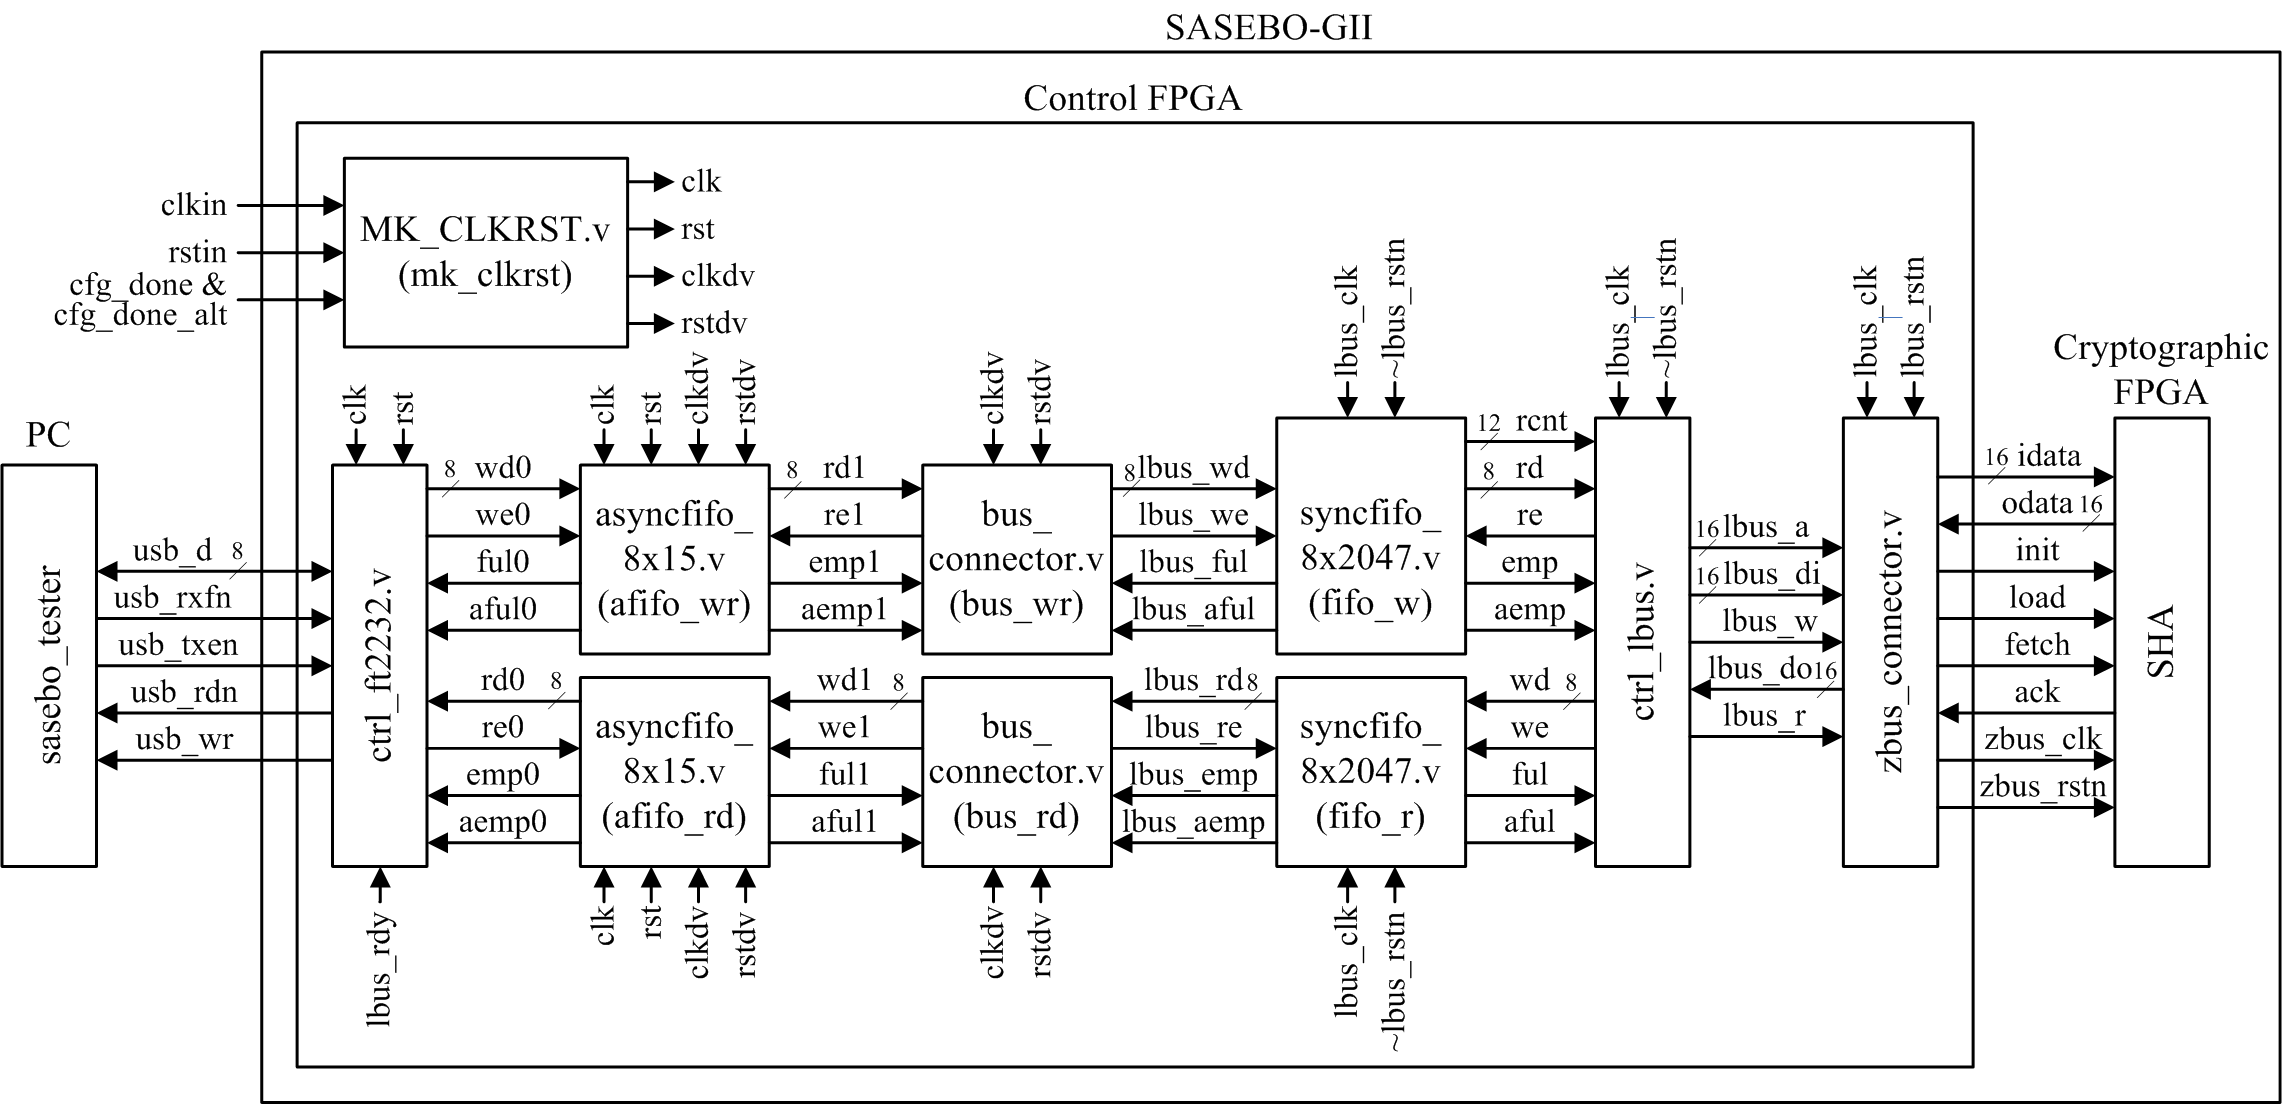
\includegraphics{img/sha3-schema.png}
    }

    \caption{Implémentation simplifié du SHA-3 sur un FPGA}
  \end{figure}
\end{frame}

\begin{frame}{Caractéristiques d'une fonction de hachage}
  \begin{block}{Le plus important : résistance aux attaques}
    Une fonction de hachage sécurisée doit être résistante à différentes attaques, telles que :

    \begin{itemize}
      \item les attaques de collisions
      \item les attaques de préimage
      \item les attaques par force brute
    \end{itemize}

    Elle doit être suffisamment robuste pour empêcher un adversaire de trouver des \textbf{collisions intentionnelles} ou de retrouver \textbf{l'entrée d'origine à partir de la valeur de hachage}.
  \end{block}
\end{frame}

\begin{frame}{Fonction de hachage : résumé}
  \begin{itemize}
    \item Une fonction de hachage prend n'importe quel mot binaire entrée et retourne un mot binaire de taille fixe
    \item Une bonne fonction de hachage possède les caractéristiques suivantes :
          \begin{itemize}
            \item Uniformité
            \item Déterminisme (= pas de hasard)
            \item Résistance aux collisions
            \item Sensibilité aux changements
            \item Efficacité
            \item \textbf{Résistance aux attaque bruteforce / reverse}
          \end{itemize}
  \end{itemize}
\end{frame}

\begin{frame}{Fonction de hachage : exercices}
  \begin{block}{Exercice 1 : se familiariser avec les fonctions de hachage}
    En CLI, calculez le hash de votre prénom / animal / n'importe quoi.
    Vous pouvez utiliser des bibliothèques ou des outils en ligne pour effectuer ce calcul.
    Comparez ensuite la valeur de hachage obtenue avec celle d'autres chaînes de caractères.
    Observez comment une légère modification de la chaîne d'entrée entraîne un changement significatif dans la valeur de hachage.
  \end{block}

  \begin{block}{Exercice 2 : calcul du hash d'un fichier}
    Calculez le hash du whitepaper du bitcoin, accessible sur \url{https://bitcoin.org/bitcoin.pdf}.
    Comparez sa valeur avec les autres.
  \end{block}
\end{frame}